%----------------------------------------------------------------------------------------
%	PACKAGES AND OTHER DOCUMENT CONFIGURATIONS
%---------------------------------------------------------------------------------------

% if you're here it means you were interested enough in me try and find our a little more. Why don't you skip the digging and go right to the source?


\documentclass[
	10pt, % Default font size, can be between 8pt and 12pt
]{FreemanCV}


% Handle images:
\graphicspath{{./images/}}


\columnratio{0.40, 0.60} % Widths of the two columns, specified here as a ratio summing to 1 to correspond to percentages; adjust as needed for your content 

% Headers and footers can be added with the following commands: \lhead{}, \rhead{}, \lfoot{} and \rfoot{}
% Example right footer:
%\rfoot{\textcolor{headings}{\sffamily Last update: \today. Typeset with Xe\LaTeX}}

%----------------------------------------------------------------------------------------

\begin{document}

\begin{paracol}{2} % Begin two-column mode

%----------------------------------------------------------------------------------------
%	YOUR NAME AND CURRICULUM VITAE TITLE
%----------------------------------------------------------------------------------------

\parbox[][0.05\textheight][c]{\linewidth}{ % Box to hold your name and CV title; change the fixed height as needed to match the colored box to the right
	\centering % Horizontally center text
	
	{\sffamily\Huge Josh \textbf{Booth}} % Your name
	
	\medskip % Vertical whitespace
	
	%{\cursivefont\Huge\textcolor{headings}{Big Bad Baller}}
	
	\vfill % Push content to the top of the box
}

%----------------------------------------------------------------------------------------
%	MAJOR RESEARCH PROJECT
%----------------------------------------------------------------------------------------

% \section{Doctral Resoearch}

% {\raggedright\textbf{``Observation of Einstein-Podolsky-Rosen Entanglement on Supraquantum Structures by Induction Through Nonlinear Transuranic Crystal of Extremely Long Wavelength Pulse from Mode-Locked Source Array"}\par}

% \medskip % Vertical whitespace

% My research examined the use of ELW pulses from a mode-locked source array inducted through transuranic crystals to observe entanglement on supraquantum structures. Theoretical advancements included prediction of quantum resonance phenomena including the possibility of resonance cascades. I was motivated to conduct this doctoral research due to my passion for teleportation of matter and I believe I have laid the foundation for further experimental validation and development of practical outcomes.

% \medskip % Extra vertical whitespace before the next section

%----------------------------------------------------------------------------------------
%	WORK EXPERIENCE
%----------------------------------------------------------------------------------------

\section{Work Experience}

% Each job is added with a \jobentry command. Below is an empty one to use as a template:

%\jobentry
%	{} % Duration
%	{} % FT/PT (full time or part time)
%	{} % Employer
%	{} % Job title
%	{} % Description

% All 5 parameters must be supplied but any can be empty if you don't need them

%------------------------------------------------

\jobentry
	{Current, from Jun 2022} % Duration
	{FT} % FT/PT (full time or part time)
	{Microchip Technology} % Employer
	{Applications/Marketing Engineer} % Job title
	{ % Description
		Bridged the gap between technical aspects of 8-bit microcontroller products and their marketing strategies.
		This role involved both developing the initial mass market campaign for multiple products
		and explaining technical concepts in an easily digestible way to the mass market and field sales reps. 
		Internally, I also lead an analytics initiative that lead to better data-driven decisions about our marketing campaign strategies.
	} 

%------------------------------------------------

\jobentry
	{Jun 2017 - Jan 2022} % Duration
	{FT/PT} % FT/PT (full time or part time)
	{United States Naval Research Laboratory} % Employer
	{Electrical Engineer Student Trainee} % Job title
	{ % Description
		Developed machine learning and a data analytic foundation through multiple projects involving
		detecting and classifying objects in satellite imagery to improve field response time,
		recovering noisy RF communications by augmenting a message passing algorithm with a Bidirectional RNN with GRU cells, 
		and identify promoter sequences in DNA using Bidirection RNN with LSTM cells.
	} 

%------------------------------------------------

\jobentry
	{Sep 2016, Jun 2022} % Duration
	{FT/PT} % FT/PT (full time or part time)
	{Booth Oil and Gas LLC.} % Employer
	{Prototype Engineer} % Job title
	{ % Description
		Developed specialized prototypes for novel problems the client faced in both day-to-day operations
		as well as for expanding the business, such as building an human-sized PEEK 3D printer for biofuel refinement.
		I offered technical expertise for project planning, cost estimation, feasibility studies.
		In addition to other project management tasks, I communicated with the client to manage their expectations
		and incorporate or remove features as their needs changed.
	}



	
%----------------------------------------------------------------------------------------
%	EDUCATION
%----------------------------------------------------------------------------------------

\section{Education} 

% Each qualification entry is added with a \qualificationentry command. Below is an empty one to use as a template:

%\qualificationentry
%	{} % Duration
%	{} % Degree
%	{} % Honors, achievements or distinctions (e.g. first class honors)
%	{} % Department
%	{} % Institution

% All 5 parameters must be supplied but any can be empty if you don't need them

%------------------------------------------------

\begin{supertabular}{r l} % Start a table with two columns, the table will ensure everything is aligned

	%------------------------------------------------
	
	\qualificationentry
		{2018-2022} % Duration 
		{Computer Engineering} % Degree
		{Summa Cum Laude; 3.98 GPA; Comp Org SI} % Honors, achievements or distinctions (e.g. first class honors)
		{Bachelors of Science} % Department
		{Shippensburg University of Pennsylvania} % Institution
	
	%------------------------------------------------
	
	\qualificationentry
		{2018-2022} % Duration
		{Mathematics} % Degree
		{} % Honors, achievements or distinctions (e.g. first class honors)
		{Minor} % Department
		{Shippensburg University of Pennsylvania} % Institution
	
	%------------------------------------------------
	

	%------------------------------------------------

\end{supertabular}

%----------------------------------------------------------------------------------------
%	PUBLICATIONS
%----------------------------------------------------------------------------------------

\section{Publications}

%------------------------------------------------

\begin{supertabular}{p{0.05\linewidth} p{0.95\linewidth}} % Start a table with two columns, the table will ensure everything is aligned
	
	%------------------------------------------------
	2023 & \href{
	https://ww1.microchip.com/downloads/aemDocuments/documents/MCU08/ApplicationNotes/ApplicationNotes/AN4889-Using-CIPs-To-Implement-Peltier-Plate-DS00004889.pdf
	}{
	AN4889: Using Core Independent Peripherals (CIPs) to Implement a Peltier Cooled Metal Plate
	\scriptsize\faLink} \\
	%------------------------------------------------
	2018 & \href{
	http://joshbooth.us/wp-content/uploads/2023/08/Machine-Learning-in-Radio-Frequency-Communications.pdf
	}{
	Machine Learning in Radio Frequency Communications
	\scriptsize\faLink} \\
	%------------------------------------------------
	2017 & \href{
	http://joshbooth.us/wp-content/uploads/2023/08/poster_SBME_promoter_predictions.pdf
	}{
	Prediction of Bacterial Promoter Sequences using Machine Learning
	\scriptsize\faLink} \\
	%------------------------------------------------
	
\end{supertabular}

\medskip % Extra whitespace before the next section

%----------------------------------------------------------------------------------------
%----------------------------------------------------------------------------------------
%----------------------------------------------------------------------------------------

% END OF COLUMN 1

%----------------------------------------------------------------------------------------
%----------------------------------------------------------------------------------------
%----------------------------------------------------------------------------------------


\switchcolumn % Switch to the second (right) column

%----------------------------------------------------------------------------------------
%	COLORED CONTACT DETAILS BOX
%----------------------------------------------------------------------------------------

\parbox[top][0.1\textheight][c]{\linewidth}{ % Box to hold the colored box; change the fixed height as needed to match the box to the left
	\colorbox{shade}{ % Create colored box and specify background color
		\begin{supertabular}{@{\hspace{3pt}} p{0.05\linewidth} | p{0.775\linewidth}} % Start a table with two columns, the table will ensure everything is aligned
			\raisebox{-1pt}{\faPhone} & (717) 494-6466 \\ % Phone number
			\raisebox{-1pt}{\small\faEnvelope} & \href{mailto:boothjmail@gmail.com}{boothjmail@gmail.com} \\ % Email address
			\raisebox{-1pt}{\small\faLink} & \href{https://joshbooth.us}{joshbooth.us} \\ % Website
			\raisebox{-1pt}{\faHome} & Chandler, AZ \\ % Address
			%\raisebox{-1pt}{\faGithub} & \href{https://github.com/username}{https://github.com/username} \\ % GitHub profile
			%\raisebox{-1pt}{\faLinkedinSquare} & \href{https://www.linkedin.com/in/username}{https://www.linkedin.com/in/username} \\ % LinkedIn profile
			% See fontawesome.pdf in the Fonts folder for all icons you can use
		\end{supertabular}
	}
	\vfill % Push content to the top of the box
}


%----------------------------------------------------------------------------------------
%	ENGINEERING PROJECTS
%----------------------------------------------------------------------------------------

\section{Notable Projects}

% Entry 0 - image on right

\subsection{DMX Light Show}

A real-time audio processing light show highlighting the flagship features on the PIC18Q71 microcontroller.
Using a single OP-AMP, it extracts 7 bands of frequencies from an audio signal using a custom band pass filter design.
It then sends lighting information over DMX to 1 of 7 nodes to create a light visualization.
Each nodes updates it's WS2812 LEDs via their SPI drivers that have been logically equated to the 1-wire protocol using CIPs.


% Entry 1 - image on left
% AI Driven Security system

\setlength\intextsep{20pt} % how far image is down from section title
\begin{wrapfigure}[7]{l}{30pt} % # of narrow lines, right top alignment, image L/R adjustment
	%\hspace*{-20pt} % how close horizontal text can be
    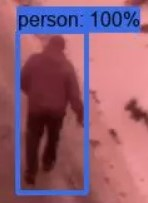
\includegraphics[width=50pt]{security_system} %Z how large image is
\end{wrapfigure}

\leavevmode \subsection{\href{https://github.com/jfcbooth/security_system}{AI-Driven Security System \scriptsize\faLink}}
%\vspace*{-5pt} % move image's anchor box up closer to title

Protoype engineer for solar-powered security system that gives real-time alerts with video anytime a classified human, vehicle, or large animal is spotted
on the property. The client also wanted all footage to be stored locally for legal purposes, so a custom program extracted motion clips
after the footage was saved, which could then be reliably transported back to a central node to do ML classification on.

% Entry 2 - image on right
% 3D PEEK Printer

\setlength\intextsep{7pt} % image in relation to subsection title
\begin{wrapfigure}[8]{rt}{25pt} % # of narrow lines, right top alignment, image L/R adjustment
	\hspace*{-23pt} % how close horizontal text can be
    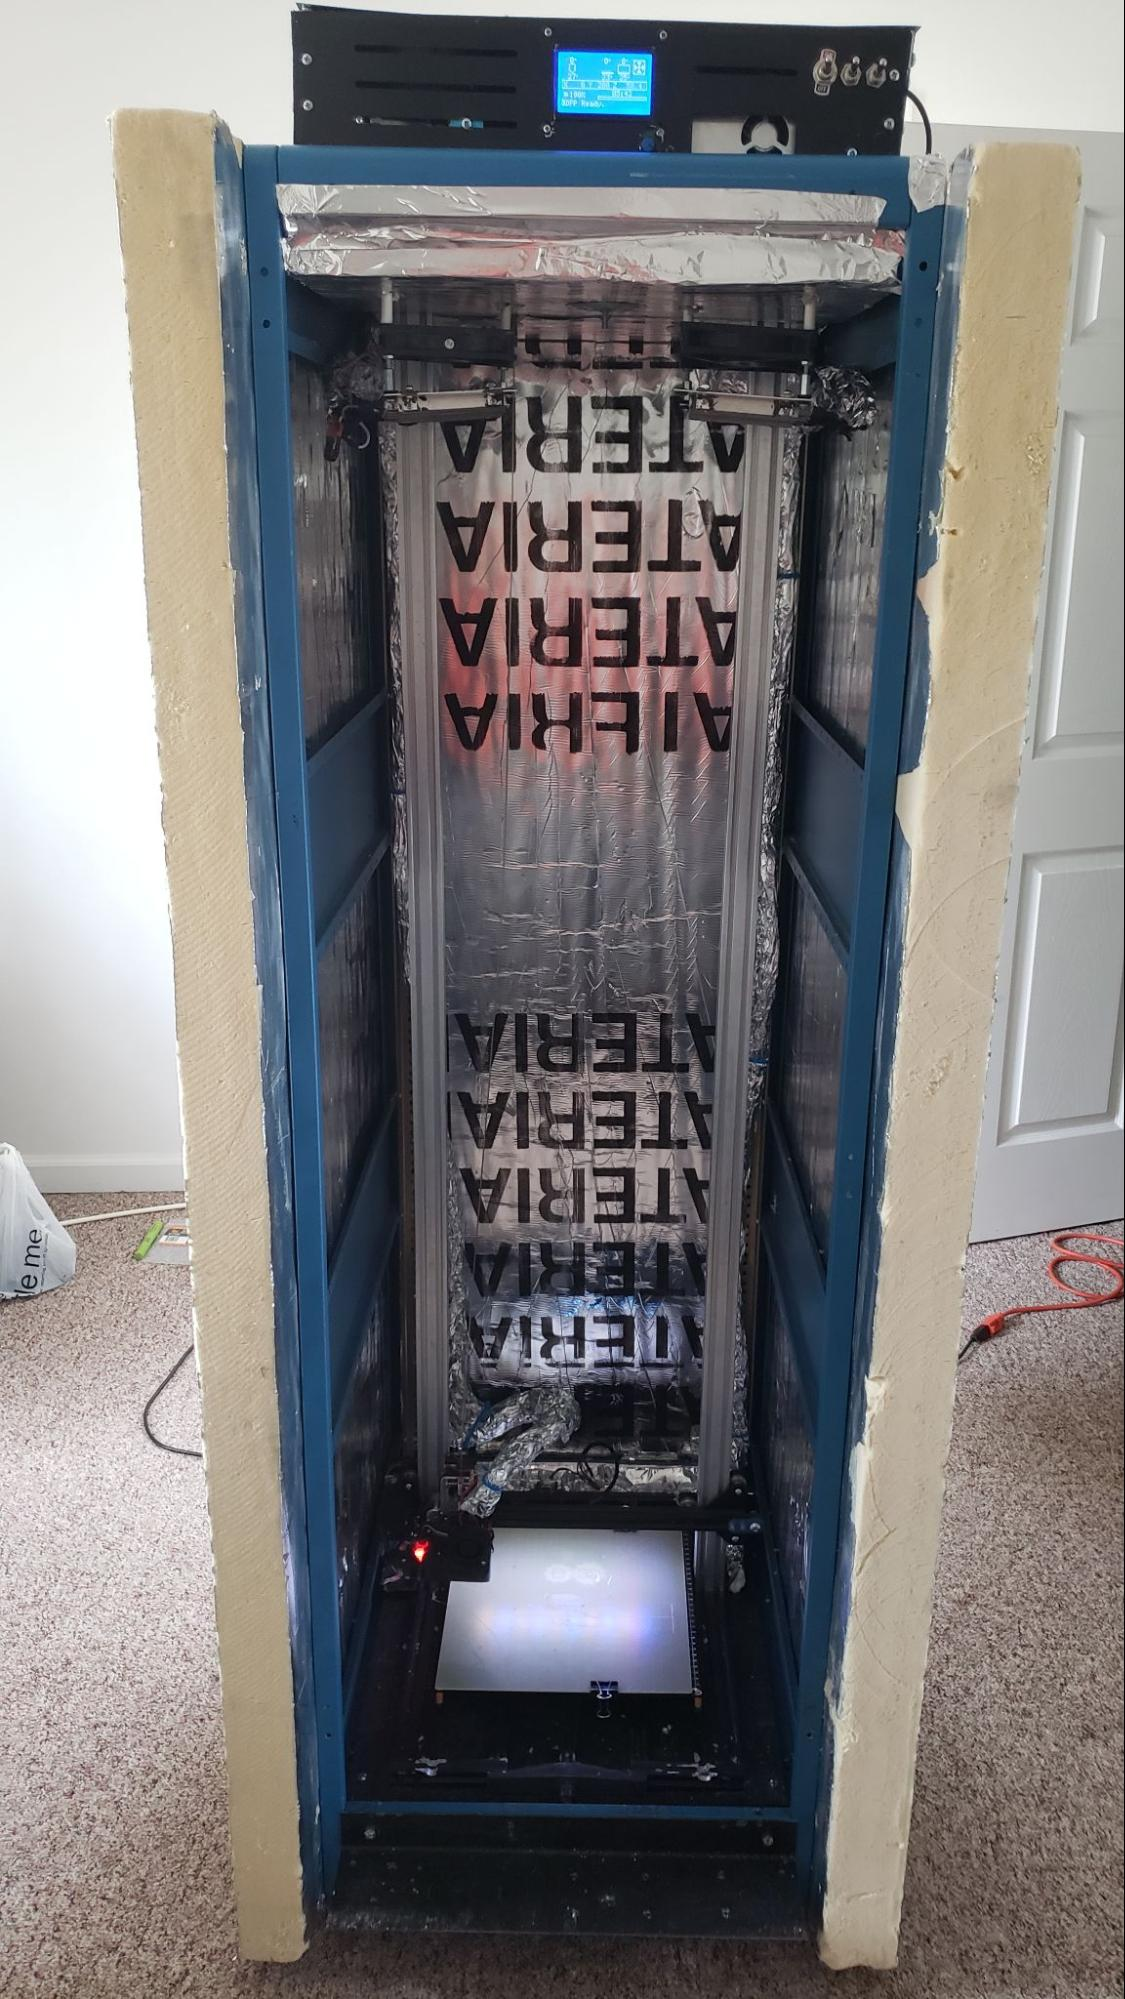
\includegraphics[width=75pt]{printer} %Z how large image is
\end{wrapfigure}

\vspace*{-10pt} % move title's anchor box up closer to title
\leavevmode\subsection{\href{https://github.com/jfcbooth/3dpp}{3D PEEK Printer \scriptsize\faLink}}

Designed and build a large-scale 3D printer capable of printing engineering-grade plastics.
This printer was specialized to print static mixers out of PEEK for biofuel refinement.
Involved in the development was designing the kinematic system, thermal dynamics, and software to safely control it's operation
while dealing with hazardous temperatures and voltages.

% Entry 3 - image on the left
% The Cold Plate

\setlength\intextsep{20pt} % how far image is down from section title
\begin{wrapfigure}[7]{l}{40pt} % # of narrow lines, right top alignment, image L/R adjustment
	%\hspace*{-20pt} % how close horizontal text can be
    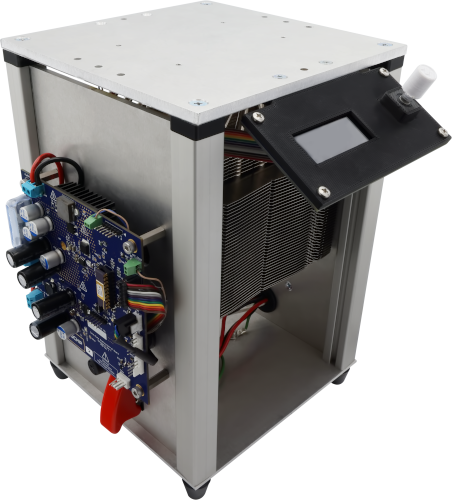
\includegraphics[width=63pt]{cold_plate} %Z how large image is
\end{wrapfigure}

\leavevmode \subsection{\href{https://github.com/microchip-pic-avr-examples/pic16f17146-cold-plate-mplab-mcc}{The Cold Plate \scriptsize\faLink}}
%\vspace*{-5pt} % move image's anchor box up closer to title

A reference design showing the most efficient way to perform the most common microcontroller tasks on a PIC16, all wrapped up into an engaging demo.
It has become Microchip's most copied code repository.


%----------------------------------------------------------------------------------------
%	AWARDS
%----------------------------------------------------------------------------------------

\section{Awards}

% This section is laid out using a table. A \tableentry command adds lines with the following parameters:

%\tableentry{Heading}{Content}{spaceafter}
% All 3 parameters must be supplied but any can be empty if you don't need them
% A "spaceafter" value in the third parameter will add some vertical space -- this is to be used between headings, leave it empty for no extra space

%------------------------------------------------

\begin{supertabular}{r l} % Start a table with two columns, the table will ensure everything is aligned
	
	%------------------------------------------------
	
	\tableentry{1985}{\textbf{Faculty of Science Masters Scholarship}}{}
	\tableentry{}{\textit{Massachusetts Institute of Technology}}{spaceafter}
	
	%------------------------------------------------
	
	\tableentry{1983}{\textbf{Top Achiever Award -- Physics}}{}
	\tableentry{}{\textit{The University of Washington}}{spaceafter}
	
	%------------------------------------------------
	
\end{supertabular}

%----------------------------------------------------------------------------------------
%	COMPUTER SKILLS
%----------------------------------------------------------------------------------------

% \section{Misc. Skills} 

% % This section is laid out using a table. A \tableentry command adds lines with the following parameters:

% %\tableentry{Heading}{Content}{spaceafter}
% % All 3 parameters must be supplied but any can be empty if you don't need them
% % A "spaceafter" value in the third parameter will add some vertical space -- this is to be used between headings, leave it empty for no extra space

% %------------------------------------------------

% \begin{supertabular}{r l} % Start a table with two columns, the table will ensure everything is aligned
	
% 	%------------------------------------------------
	
% 	\tableentry{Beginner}{Java, MS DOS}{spaceafter}
	
% 	%------------------------------------------------
	
% 	\tableentry{Intermediate}{Javascript, Python, HTML, CSS,}{}
% 	\tableentry{}{Microsoft Windows}{}
% 	\tableentry{}{Computer Hardware \& Support}{spaceafter}
	
% 	%------------------------------------------------
	
% 	\tableentry{Expert}{Perl, Unix, \LaTeX}{spaceafter}
	
% 	%------------------------------------------------
	
% \end{supertabular}

%----------------------------------------------------------------------------------------
%	COMMUNICATION SKILLS
%----------------------------------------------------------------------------------------

% \section{Communication Skills}

% % This section is laid out using a table. A \tableentry command adds lines with the following parameters:

% %\tableentry{Heading}{Content}{spaceafter}
% % All 3 parameters must be supplied but any can be empty if you don't need them
% % A "spaceafter" value in the third parameter will add some vertical space -- this is to be used between headings, leave it empty for no extra space

% %------------------------------------------------

% \begin{supertabular}{r l} % Start a table with two columns, the table will ensure everything is aligned
	
% 	%------------------------------------------------
	
% 	\tableentry{Conferences}{Oral Presentation at the Annual MIT}{}
% 	\tableentry{}{Theoretical Physics Conference -- 1987}{spaceafter}
	
% 	%------------------------------------------------
	
% 	\tableentry{Posters}{Poster at the Meeting of the American}{}
% 	\tableentry{}{Physical Society -- 1985}{spaceafter}
	
% 	%------------------------------------------------
	
% \end{supertabular}

%----------------------------------------------------------------------------------------

\end{paracol} % End two-column mode

%----------------------------------------------------------------------------------------

\end{document}
